\chapter{Praktiskā daļa}\label{sec:prakt}
Šajā nodaļā, lai novērtētu mobilitātes ietekmi uz pakalpojuma kvalitāti bezvadu sensoru tīklos, aprēķiniem tiks izmantota lietojumprogramma MATLAB un \ac{NS-2} v.2-35. MATLAB ir izmantots BER līmeņa analīzei statiskā WSN tīkla kanālā, lai vēlāk šos datus saildzinātu ar NS-2 iegūtajiem rezultātiem.
Visās datorsimulācijās tika izmantoti tīkli ar vienādām fiziskā slāņa īpašībām. Pielikumā var apskatīt izmantoto NS-2 šablonu (\seename~\ref{appen:NETtempl}). Simulācijas parametri apkopoti Tab.\ref{tab:param}, maksimālā pārraides jauda un uztvērēja jūtīgums atbilst Lucent’s WaveLAN parametriem, tehnoloģija kuru iespējams pielietot WSN tīklu izveidei.
\begin{table}[!htb]
\centering
 \begin{tabular}{|l|c|c|}
\hline
~&\multicolumn{2}{c|}{Lucent’s WaveLAN}\\
\hline\hline
mezglu skaits&\multicolumn{2}{c|}{51}\\\hline
Tīkla laukums [$m\times m$]&1500$\times$300&500$\times$300\\\hline
Viļņu izplatīšanas veids&\multicolumn{2}{c|}{Two Ray Ground}\\\hline
Antenas veids&\multicolumn{2}{c|}{omnidirectional}\\\hline
Frekvence [MHz]& \multicolumn{2}{c|}{915}\\\hline
Raidītāja jauda [W]&\multicolumn{2}{c|}{0.001}\\\hline
Pārraides ātrums &2 [Mbit/s]&40 [Kbit/s]\\\hline
Radiouztvērēja slieksnis [W]&\multicolumn{2}{c|}{3.652$\times10^{-13}$}\\\hline
%Treshold to avoid collisions [W]&\multicolumn{2}{c|}{1.559x$10^{-11}$}\\\hline
Kolīziju slieksnis [dB]&\multicolumn{2}{c|}{10}\\\hline
MAC protokols& \multicolumn{2}{c|}{802.11}\\\hline
Traffika veids&\multicolumn{2}{c|}{CBR}\\\hline
Paketes garums [biti]&\multicolumn{2}{c|}{512}\\\hline
Pakešu izveides ātrums [pck/s]&\multicolumn{2}{c|}{4}\\\hline
Maršrutēšanas protokols&AODV&DSR\\\hline
Pakešu skaits rindā&\multicolumn{2}{c|}{64}\\\hline
Simulācijas laiks [s]&\multicolumn{2}{c|}{900}\\\hline
$t_{pause}$ [sek] &\multicolumn{2}{c|}{0, 30, 45, 60, 120, 300, 450, 600, 900}\\\hline
Komutācijas veids&\multicolumn{2}{c|}{NRBS}\\\hline
Mobilitātes Modelis&\multicolumn{2}{c|}{RWMM}\\\hline
$max$ mezglu ātrums [m/s]&\multicolumn{2}{c|}{0, 5, 10, 15, 20}\\
\hline
\end{tabular}
\caption{Simulācijas parametri}
\label{tab:param}
\end{table}

\section{Raiduztvērēju parametri}
Lai sasniegtu reālistiskos rezultātus tiek izmantoti reālo raiduztvērēju un raidītāju  parametri: Lucent’s WaveLAN frekvences ir $f_{c}$ = 915 MHz un raidītāj jauda $P_{t}$ ir 1mW.

\subsection{Radiouztvērēja slieksnis}
Ar radiouztvērēja slieksni $RXThresh\_$ raksturo minimālo jaudu kas ir nepieciešama veiksmīgai paketes saņemšanai. Lucent’s WaveLAN radiouztvērēja jutīgums ir -94 dBm, tātad $RXThresh\_$ = -94 dBm kas ir 3.981$\times10^{-13}$ W.\\
NS-2 vidē, ja pakete nonāk mezglā ar jaudu, kas ir lielāka vai vienāda ar slieksni, tad tiek uzskatīts, ka sūtītājs atrodas pārraides apgabalā un pakete ir veiksmīgi saņemta.

\section{MATLAB}
Mobilitātes apstākļos datu pārraidei ir nepieciešams nodrošināt divus nosacījumus: 1) mezgla A raidītājapgabalā ir jābūt uztvērēj-mezglam un 2) mezgliem jābūt vienam otra uztveršanas diapazonā  laika periodā $t$, lai pārraidītu $M$ garu ziņojumu pie datu pārraides ātruma $R_{b}$.

\subsection{Datu pārraides ātrums un mezglu kustības ātrums}
Savienojuma ilgumam jābūt tādam, lai laikā brīdi $t_{par}$ kaut vienu reizi nosūtīt ziņojumu uztvērēj-mezglam. Šo laika brīdi nosaka mezglu kustības ātrums un uztvērēj-mezgla jūtīgums, kā arī datu pārraides ātrums. Pie radiouztvērēja jutīguma -94 dBm, ideālos apstākļos kad interference netiek ņemta vērā, maksimālā distance pie kuras uztvērēj-mezgls saņems ziņojumu bez kļūdām  ir $r_{range}$ = 6.43 m (saskaņā ar (\ref{eq:r_range}) vienādojumu). Lai vienkāršot aprēķinus tiek pieņemts, ka divi mezgli kustas viens otram pretī ar vienādiem ātrumiem un sāk un pabeidz datu pārraidi $r_{range}$ attālumā no uztvērēj-mezgla (\seename ~\figurename. ~\ref{fig:mezgli}).

\begin{figure}[!htb]
\centering
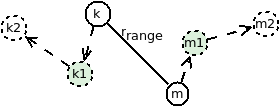
\includegraphics[scale=0.6]{./graph/mezgli.png}
\caption{Mezglu kustība}
\label{fig:mezgli}
\end{figure}

Tad laiks nepieciešams šķērsot šo attālumu pie mezglu vidējā ātruma no 5 līdz 20 [m/s] intervālā, būs vienāds ar

\begin{table}[!htb]
\centering
\begin{tabular}{|l|l|}
\hline
Vid. ātrums [m/s]&Laiks [s]\\\hline
5&1.286\\
10&0.643\\
15&0.428\\
20&0.321\\\hline
\end{tabular}
\caption{Laks lai šķērsot $r_{range}$ distanci pie dažādiem ātrumiem}\label{tab:atrumi}
\end{table}

Tagad zinot laika intervālu, var aprēķināt paketes skaitu ko mezgls nosutīs pie dažādiem datu pārraides ātrumiem.
\begin{figure}[!htb]
\centering
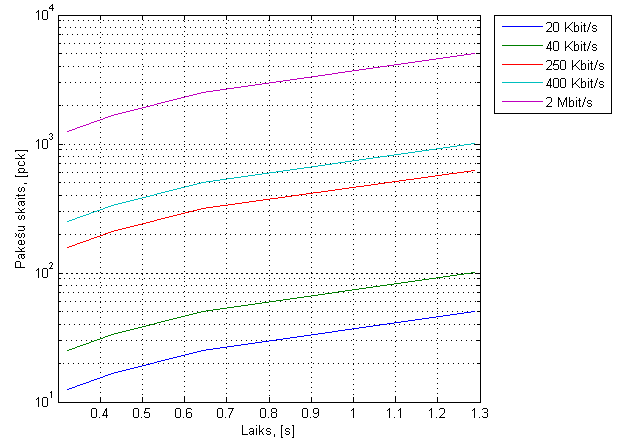
\includegraphics[scale=0.7]{./graph/vpck.png}
\caption{Pakešu skaits atkarība no datu pārraides ātrumiem}\label{fig:speed}
\end{figure}
Attēlā \ref{fig:speed} pieņemts ka paketes garums ir 512 biti, pakešu skaits būs atkarīgs no lietojumprogrammas. Lai iegūt pēc iespējas pilnīgu priekšstatu par tīkla darbību tiek pieņemts, ka datu pārraides ātrums ir 2 Mbit/s (augšēja robeža).

\subsection{Blīvuma ietekme}
Mezglu kustību var sadalīt relatīvi mazos laika posmos $\delta$t, tādos laika intervālos mobilo mezglu kustība būs tuva nullei (0). Un mobilo tīklu var apskatīt kā stacionāru. Izmantojot aprēķinu metodi (\seename ~\ref{sec:moby} sadaļu) tiek aprēķināta likumsakarība starp BER līmeni daudzposmu maršrutā un mezglu telpisko blīvumu tīklā. MATLAB programmu var apskatīt pielikumā (sk.~\ref{appen:matlabBERdensity})
\begin{figure}[!htb]
  \centering
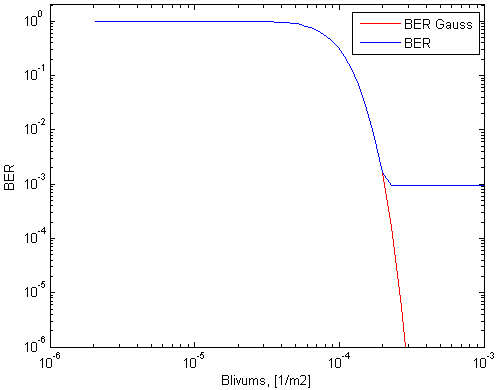
\includegraphics[scale=0.7]{./graph/blivBER.png}
\caption{BER daudzposmu maršrutā beigās atkarība no mezglu telpiska blīvuma tīklā}\label{fig:bliv}
\end{figure}

Attēlā \ref{fig:bliv} parādīta BER vērtībā atkarībā no mezglu izkliedes tīklā, kur sarkanā līnija ir $BER_{Gauss}$, kas ir aprakstīta šī darba \ref{sec:moby} sadaļā un zilā atbilst G.Ferrati un O.Tonguz piedāvātai metodei \cite{qoS_mobility} kurā, kad $\rho\rightarrow\infty$  tad $BER_{link} \simeq \frac{3\lambda M}{4R_{b}}$. Un $BER_{route}$ būs
\begin{equation}
 BER_{route}\simeq max \left \{  \left[ 1- \left[1-Q\left(\sqrt {\frac{2Pr}{Ptherm+Pini}}\right)\right]^{n_{h}}\right], \frac{3n_{h}\lambda M}{4R_{b}}\right \},
\end{equation}
kur $M$ ir ziņojuma garums.

Kā jau iepriekš tika minēts - lai izveidotu savienojumu ir nepieciešams uztvērēj-mezgls raidīšanas diapazonā laika periodā $t_{par}$. Pie zema $\rho_{s}$ BER līmenis daudzposmu maršruta beigās ir gandrīz viens (1), tādēļ tā raidītā jauda ir nepietiekami augsta lai pārraidītu signālu tik lielā attālumā. Savukārt pie $\rho_{s}$ ap  $5\times10^{-4}$ tas pazeminās, šajā robežā uztvērēj-mezgla jutīgums ir pietiekami augsts lai uztvert signālu, turklāt interference no apkārt esošiem mezgliem ir niecīga. Savukārt ar $r_{link}$ ($r_{link}=1/\sqrt{\rho_{s}}$) pazemināšanu kanālā palielinās interferences un tas ir galvenais trokšņu avots.
Ņemot vērā iepriekš teikto šajā darbā NS-2 realizētajos scenārijos būs apskatīts tīkls ar telpisko blīvumu $\sim10^{-4}$ lai izslēgtu varbūtību, ka datu pārraide tiek traucēta kāda cita iemesla dēļ.


\section{NS-2 simulācijas}
\acf{NS-2} lietojumprogramma ir diskrēto notikumu modelējoša (discrete event simulator) programma, kas bieži tiek izmantota telekomunikāciju tīklu pētījumos. Ar NS-2 iespējams modelēt TCP, maršrutēšanas un multiraides protokolu darbību vadu un bezvadu (WLAN, WPAN un satelīt) tīklos \cite{ns2}.

Maģistra darbā izmantoto NS-2 simulāciju scenāriju pilns apkopojums ir iekļauts maģistra darbam pievienotajā CD - ''Maģistra darbā ''Mobilitātes ietekme uz pakalpojuma kvalitāti sensoru tīklos'' izstrādātie NS-2 simulāciju scenāriji''.


\subsection{Datorsimulācijas parametri}

\subsubsection{Kolīziju slieksnis}
Datu pārraides laikā var gadīties, ka galamērķī vienlaicīgi pienāk divas paketes, izraisot kolīziju. NS-2 vidē kolīziju potenciāli var izraisīt tikai paketes ar jaudu, kas ir augstāka par $RXThresh\_$. Ja abām paketēm jaudas ir augstākas par $RXThresh\_$, tad to jaudu attiecības tiek salīdzinātas ar kolīziju slieksni $CPThresh\_$. Šajā eksperimentā kolīziju slieksnis tiek pieņemts $CPThresh\_$ = 10 dB.

\subsubsection{Viļņu izplatīšanās veids}
Tiek uzskatīts, ka tīkls ir plakana virsma un visi mezgli kustās tikai X un Y koordinātēs. Līdz ar to, lai sasniegtu iespējami reālistiskus rezultātus, tiks izmantots ''two-ray ground'' modelis. Šajā modelī uztvertā jauda tiek raksturota ar Friis formulu (\seename (~\ref{eq:pr}) formulu) ar $\gamma$ = 4.  Two-ray ground modelī mezgls uztver gan atstaroto signālu gan arī to, kas nonāk līdz mezglam bez atstarojuma. Lai izmantotu šo modeli NS-2 mezglu antenām ir jābūt izvietotām vienādā augstumā, tāpēc visos scenārijos tiek pieņemts, ka Z = 1.5 m.

\subsubsection{MAC protokol}
IEEE 802.11 standartā, RREQ paketes tiek pārraidītas apraides (broadcast) veidā, savukārt RREP un RERR un  datu pakešu pārraide notiek uniraides  veidā, šāda tipa paketes ir adresētas noteiktiem kaimiņ-mezgliem. Savienojuma pārrāvums tiek konstatēts ar MAC līmeņa palīdzību. Kad MAC līmenis uniraides paketes posmā otram mezglam vairs nespēj piegādāt paketes, tad uz maršrutēšanas līmeni tiek nosūtīts signālziņojums. Piemēram, gadījumos kad pēc datu pārraides beigām netiek saņemta ACK pakete.

\subsubsection{Buferis}
Visi šajā nodaļā apskatītie maršrutēšanas protokoli uztur nosūtīšanas buferi, kura garums ir 64 paketes. Paketes, kurām maršruta atklāšanas (route discovery) process ir ticis iniciēts, taču mezglā vēl nav saņemta RREP pakete, tiek ievietotas buferī. Gadījumā, kad pakete atrodas buferī ilgāk par 30 sek. tā tiek dzēsta. Līdz mirklim kad MAC līmenis atkal būs pieejams gan datu, gan maršrutēšanas paketes tiek ievietotas rindas interfeisā (interface queue). Rindas interfeisa garums ir 64 paketes un tajā maršrutēšanas protokoliem ir prioritāte, visas parējās paketes tiek sūtītas rindas kartībā.

\subsubsection{Trafiks un Mobilitātes modelis}
Šajā simulācijā tika izmantots konstants bitu ātruma (\acs{CBR}) avots, ar konstantu pakešu izveides ātrumu $\lambda$ [pck/s]. Avots-galamērķis pāris ir nejauši izvietots tīkla laukumā. NS-2 standart pakā ir iebūvēta \texttt{cbrgen.tcl} utilītprogramma trafika automātiskai izveidei. Ar šo utilītprogrammu tika izveidoti CBR trafika šabloni, kas savukārt turpmākajā darbā tika izmantoti kā ievaddati. Visās simulācijas mezglu mobilitātei ir izmantots (\acs{RWMM}) (\seename nodaļa ~\ref{sec:mobilityModels}). \acf{RWMM} mezgli kustas ar gadījuma ātrumu [$v_{min}, v_{max}$] līdz gadījuma mērķim. Simulācijas mērķis bija noteikt mezglu mobilitātes ietekmi uz QoS pie dažādiem ātrumiem. Visu simulāciju ilgums ir 900 sek. un simulācijas sakumā katrs mezgls ir nekustīgs $t_{pause}$ laika periodu.
Pauzes laiks $t_{pause} = 0$ atbilst nepārtrauktai mezglu kustībai (saskaņā ar RWMM modeli), savukārt $t_{pause} = 900$ sek. atbilst stacionāram tīklam kurā kustības nav, jo pauze ilgst visu simulāciju. RWMM kustības šablona izveidošanai tika izmantota NS-2 iebūvētā utilītprogramma \texttt{setdest.tcl}.

\subsubsection{Enerģija modelis}
Enerģijas modelis ir iebūvēts NS-2 kā mezglu atribūts. Enerģijas modelī ir ''initial value'' kas atbilst enerģijas līmenim darbības sakumā un pēc katras paketes pārraides/saņemšanas tas ņem vērā ar to saistīto enerģijas patēriņu. Kad mezgla enerģijas līmenis sasniedz nulli, mezgls ''nomirst'', tas vairs nevar saņemt, retranslēt vai nosūtīt paketes. Šajā darbā enerģijas patēriņš netiek ņemts vērā.


\subsection{Veiktspējas analīzes parametri}
Šajā darbā tiek pētīta mobilitātes ietekme uz servisa kvalitāti WSN tīklā. QoS līmenis ir noteikta prasību kopa kuru tīklam ir jānodrošina pārraidot datus no avota līdz galamērķim. Mobilitātes un dinamiskās topoloģijas dēļ, kā arī dēļ fiziskā slāņa ierobežojumiem var gadīties, ka tīkla resursi ne vienmēr ir pieejami pilnā apjomā visu pakešu vienlaicīgai pārraidīšanai. Līdz ar to, tādi parametri kā, piemēram, caurlaidspēja, aizkavē pakešu izmešanu (packet drop) un tam ir jāpievērš pastiprināta uzmanība. Lai noteiktu pakalpojumu kvalitāti stacionārā un mobilā WSN tīklā, tika izmantoti sekojoši veiktspējas parametri. \ac{PDF} un vidējā aizkave tīklā ir vieni no svarīgākajiem parametriem veiktspējas analīzē.

\subsubsection{\acl{PDF}}
\acf{PDF} ir attiecība starp veiksmīgi saņemtām CBR paketēm un summu visu izveidoto CBR pakešu simulācijas laikā. Tas ir svarīgs parametrs kas norāda uz tīkla pārblīvi\footnote{Pārmērīgi intensīva ziņojumu plūsmu, kas aizkavē ziņojumu pārsūtīšanu datoru tīklā, nelabvēlīgi ietekmē datoru tīkla veiktspēju un var radīt pārraidāmās informācijas zudumus \cite{lza}.} tīklā. PDF palīdz raksturot protokola veiktspēju vadoties pēc pakešu pazaudēšanas koeficienta (packet loss rate), ko ietekmē tādi faktori kā paketes garums, tīkla noslodze un mainīga topoloģija. Augsts PDF lielums nozīmē, ka pazaudētu pakešu skaits ir zems un no datu nosūtīšanas viedokļa protokols ir efektīvs. Šeit ir svarīgi atzīmēt, ka pie augsta PDF pakete, kas saņemta ar lielu aizkaves laiku ir nederīga. PDF un laika aizkave ir vienādi svarīgi parametri.
\begin{equation}
 PDF=\frac{\sum Sa_{CBR}}{\sum No_{CBR}},
\end{equation}
kur $Sa_{CBR}$ ir visās veiksmīgi saņemtas CBR paketes un $No_{CBR}$ ir visas nosūtītās CBR paketes.

\subsubsection{Vidēja aizkavē tīklā}
Vidējā aizkave tīklā, jeb abpusējā aizkave (end-to-end delay), ir vidējā laika starpība starp laika brīdi kurā paketi tika izveidota avotā, līdz brīdim kad tā tika saņemta galamērķī. Pazaudētās paketes netiek ņemtas vērā. Savukārt, tiek ņemtas vērā aizkaves kas ir radušās dēļ maršruta atklāšanas (route discovery), atkārtotām pārraidēm,  gaidīšanas laika rindā un viļņu izplatīšanās laiks. Visu savienojumu aizkaves tiek summētas kopā un tiek dalītas ar izveidoto savienojumu skaitu visas simulācijas laikā.
\begin{equation}
Avg.delay=\frac{\sum( Laiks_{gal} - Laiks_{avots})}{\sum N_{sav}},
\end{equation}
kur $Laiks_{gal}$ ir laika brīdis kurā pakete nonāk galamērķī, $Laiks_{avots}$ ir laika brīdis, kurā avots izsūtīja šo paketi un $N_{sav}$ ir savienojumu pāru skaits tīklā.

\subsubsection{Caurlaidspēja}
Tīkla caurlaidspēja ir datu daudzums kas vienas sekundes laikā tiek pārraidīts no avota uz galamērķi. Analizējot iegūtos datus tika ņemtas vērā tikai CBR paketes, ignorējot papildus tēriņus - tādus kā HELLO, RREQ un RREP utt.. Tika aprēķinātas divas caurlaidspējas: 1) mezgla caurlaidspēja - attiecība starp mezglā veiksmīgi saņemtu pakešu skaitu pret kopējo bitu skaitu simulācijas laikā. 2) Tīkla caurlaidspēja, kas ir vidējā mezglu caurlaidspēja tīklā - skaitot tikai tos mezglus, kas ir iesaistīti CBR datu pārraidē.
\begin{equation}
 n_{through}=\frac{\sum n_{bit}}{t_{sim}},
\end{equation}
kur $\sum n_{bit}$ ir summārais mezglā saņemto bitu skaits un $t_{sim}$ ir simulācija ilgums.
\begin{equation}
Tīkla.caurlaidspēja =\frac{\sum n_{through}}{N},
\end{equation}
kur $ \sum n_{through}$ ir visu mezglu summārā caurlaidspēja un $N$ ir  kopējais mezglu skaits tīklā.


\section{Rezultātu analīzē}
Simulācijas laikā iegūte rezultāti raksturo procesus tīklā ar telpisko blīvumu $\rho_{s} = 1.13\times10^{-4}$, distance starp raidītājmezglu līdz uztvērējmezglu ir $r_{link} = 134.2$ m un 10 no 51 mezgla ģenerē datus. Lai visi simulāciju scenāriju būt pēc iespējas vienādi, stacionārā tīkla mezglu izvietojums tika izveidots pēc tā pāša principa kā pārējie, ar tādu atšķirību, ka mezglu ātrums vienāds ar 0.01 [m/s] un pauzes laiks vienāds ar 900 sekundēm.

\subsection{Paketes piegādes sadale un vidējā aizkava tīklā}
\begin{figure}[htb!]
\begin{minipage}[t]{0.47\linewidth}
\centering
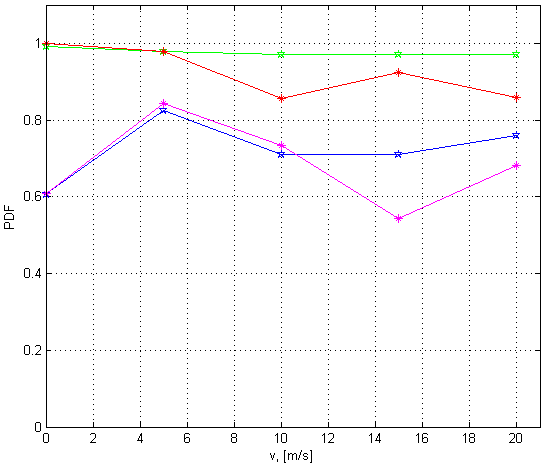
\includegraphics[scale=0.55]{./graph/vPDF.png}
\caption{Paketes piegādes sadales atkarība no maksimālā ātruma}
\label{fig:pdfspeed}
\end{minipage}%
\hspace{0.2cm}
\begin{minipage}[t]{0.47\linewidth}
\centering
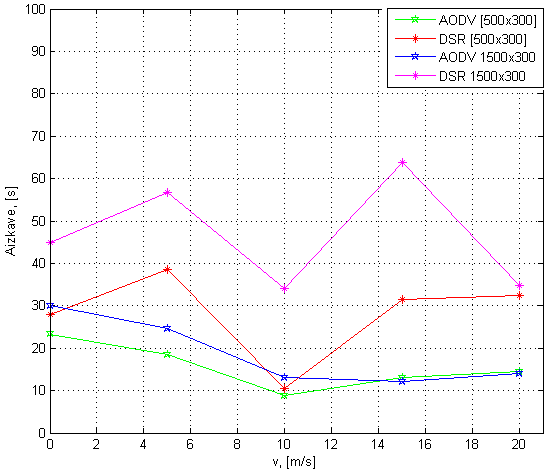
\includegraphics[scale=0.55]{./graph/vDelay.png}
\caption{Vidējā aizkave tīklā atkarībā no maksimālā ātruma}
\label{fig:avgDspeed}
\end{minipage}
\end{figure}
Attēlā \ref{fig:pdfspeed} parādīta PDF atkarība no maksimālā mezglu ātruma ar AODV un DSR maršrutē-šanas protokoliem, un tīkla telpiskā blīvuma $\rho_{1500\times300}$ = 1.13$\times10^{-4}$ un $\rho_{500\times300}$ = 3.4$\times10^{-4}$, [$\frac{1}{m^{2}}$]. Pie $\rho_{500\times300}$ = 3.4$\times10^{-4}$ stacionārā tīklā PDF ir gandrīz vienāds ar 1. Ar kustības sākumu tas degradē, it sevišķu gadījumos, kad tiek pielietots DSR protokols, pie maksimālā ātruma 20 [m/s] tas tuvinās pie 0.8 (datu piegāde krīt par $\sim$17\%). Savukārt pie $\rho_{1500\times300}$ = 1.13$\times10^{-4}$ stacionāram tīklam PDF ir vienāds tikai ar 0.6 un mezglu mobilitātes apstākļos tā pieaug vidēji par $\sim$12\%, sasniedzot maksimumu pie ātruma 5 [m/s]. PDF pārsniedz 0.8.

Kā var redzēt attēlā \ref{fig:pdfspeed} maršrutēšanas protokola izvēle lielā mērā ietekmē kopējo tīkla veiktspēju mobilitātes apstākļos. Ar mezglu ātrumu pieaugumu DSR protokols uzrāda aizvien sliktākus rezultātus salīdzinājumā ar AODV. Tas ir izskaidrojams ar to ka DSR protokols ir distances vektora protokols un mezgls savā kešatmiņā uztur datus tikai par maršrutiem līdz 1. kārtas kaimiņ-mezgliem. Jo straujāk mainās topoloģija (šajā gadījumā jo ātrāk kustas mezgli) jo vairāk DSR maršrutēšanas pakešu nepieciešams lai izveidotu datu pārraidi.

Daudzas lietojumprogrammas piegādātās paketes ar lielu laika aizkavi tiek uzskatītas per nederīgām. Attēls \ref{fig:avgDspeed} ilustrē tīkla vidējās aizkaves izmaiņas atkarībā no mezglu maksimālā kustības ātruma. Viszemākā aizkave tīkla ir pie maksimālā ātruma 10 [m/s]. Tas nozīmē, ka pie mezglu maksimālā kustības ātruma 10 [m/s] (vidēja 7.5 [m/s], no \texttt{trace} failā). Salīdzinājumā ar statisko tīklu pie $\rho_{500\times300}$ = 3.4$\times10^{-4}$ mobilitāte ļauj samazināt vidējo pakešu aizkavi pat 2 reizes. Savukārt AODV atkal uzrāda labākus rezultātus salīdzinājumā ar DSR. Mobilitātes apstākļos AODV spēj nodrošināt datu maršrutēšanu ar vidējo aizkavi tīklā ne augstāku par 15 sekundēm (kad mezglu maksimālais ātrums pārsniedz 5 [m/s]). Tas ir saistīts ar to ka informācija par tīkla topoloģiju izplatās daudz ātrāk nekā stacionārā.

\subsection{Caurlaidspēja}
\begin{figure}[!htb]
\centering
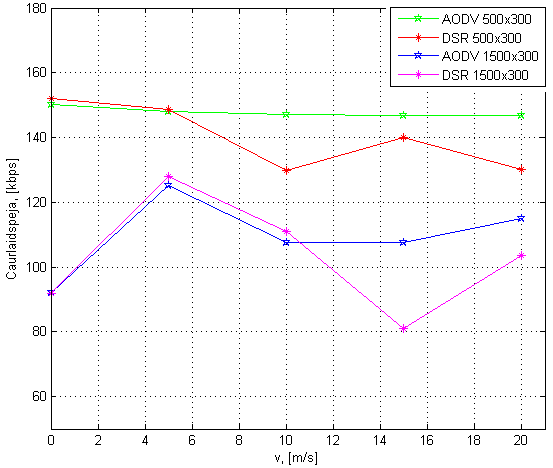
\includegraphics[scale=0.75]{./graph/vThrough.png}
\caption{Tīkla vidēja caurlaidspēja atkarība no maksimālā ātruma}
\label{fig:avgT}
\end{figure}
Kā var redzēt attēla  \ref{fig:avgT} pie mezglu telpiskā blīvuma 3.4$\times10^{-4}$ tīkla vidējā caurlaidspēja samazinās un tam ir loģisks izskaidrojums - pieaug maršrutēšanas pakešu skaits, kas ir nepieciešams datu pārraides izveidošanai. Savukārt, pie $\rho_{1500\times300}$ = 1.13$\times10^{-4}$ tīkla vidēja caurlaidspēja pieaug salīdzinājumā ar tā paša tīkla statisko modeli. Līdz ar to ir iespējami divi izskaidrojami, pirmkārt datu pārraide pieaug tādēļ ka kustīgi mezgli spēj ātrāk piegādāt datus līdz galamērķim. Gadījumā kad mezgli ir izkliedēti tīkla, mezglu kustība ļauj ātrāk pārvietot informāciju telpā, neatkarīgi no maršrutēšanas protokola. Savukārt pie 3.4$\times10^{-4}$ mobilitāte traucē it sevišķi DSR protokola izmantošanas gadījumā.

Ņemot vērā mezglu izkliedes pakāpi, vislabākos rezultātus uzrād AODV protokols pie $\rho_{1500\times300}$ = 1.13$\times10^{-4}$ vidēji paaugstinot tīkla caurlaidspēju par 15 [Kbit/s], kas ir aptuveni 18\% no stacionārā tīkla.

\subsection{AODV protokola veiktspēju atkarība no pauzes laika}
Iepriekšējā sadaļā bija apskatīta AODV un DSR protokolu darbība tīklā  ar nepārtraukti kustošiem mezgliem. Savukārt, ja gribam iegūt labāku priekšstatu par mobilitātes ietekmi uz tīkla darbību, tad ir nepieciešams novērtēt kustības maiņas ietekie. Gadījuma maršrutpunktu mobilitātes modelī mezgls sasniedzot savu galamērķi var uztaisīt pauzi uz kādu  $t_{pause}$ laiku, šajā laikā brīdi mezgla ātrums $v$ vienāds ar 0. Pēc pauzes mezglam tiek piešķirts jauns ātrums un jauns galamērķis. Lai uzzinātu kā AODV protokols spēj darboties pie dažādām mobilitātes pakāpēm, $t_{pause}$ tiek piešķirti sekojošas vērtības [0, 30, 45, 60, 120, 300, 450, 600, 900] sekundes un ar $\rho_{1500\times300}$ = 1.13$\times10^{-4}$.

\begin{figure}[htb!]
\begin{minipage}[t]{0.47\linewidth}
\centering
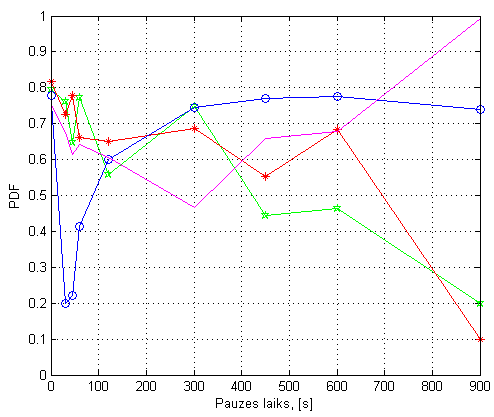
\includegraphics[scale=0.55]{./graph/pdf.png}
%\caption{Paketes piegādes sadale atkarība no pauzes laika}
%\label{fig:pdf}
\end{minipage}%
\hspace{0.2cm}
\begin{minipage}[t]{0.47\linewidth}
\centering
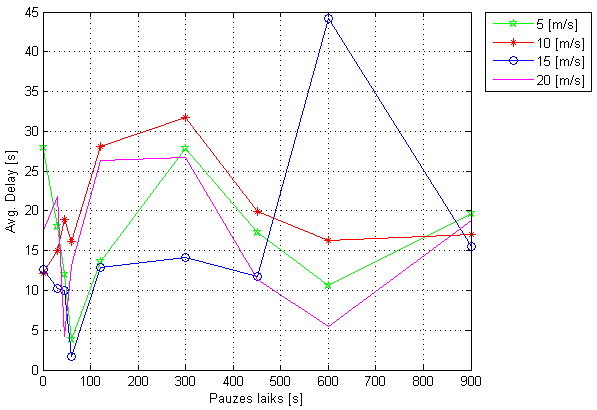
\includegraphics[scale=0.55]{./graph/avgD.png}
%\label{fig:avgD}
\end{minipage}
\caption{Vidēja aizkavē tīklā atkarība no pauzes garuma}\label{fig:pause}
\end{figure}
Attēlā \ref{fig:pause} pāradīta AODV protokola veiktspēja kā funkcija no pauzes garuma. Pie augstas mobilitātes, kad $t_{pause}$ ir zemāka par 300 sekundēm, salīdzinājumā ar $t_{pause}$ = 0 notiek aptuveni 15\% PDF kritums, savukārt, vidējā aizkave samazinās divas reizes pie $t_{pause}$ [30 - 120] sek. No kā var secināt, ka pauzes intervāls 60 sekundes (aizkavē mazāk nekā 5 sekundes) ir laiks kas ir nepieciešams AODV lai pielāgotu maršrutu. Par jebkurām izmaņām maršrutā ir jāmaksā ar datu pārraides daudzumu un pie $t_{break}$ = 60 PDF samazinās par 10\%. AODV maršrutēšanas paketēm ir prioritāte rindā. Šeit ir svarīgi atzīmēt ka, scenārijā pakešu garums ir 512 biti un tie ražoti ar ātrumu 4 pck/s, kas kopumā rāda augstu tīkla noslodzi. Kā arī mezglu izvietojums tīkla laukumā, koordinātēs X un Y ir gadījuma lielumi, un būtiski ietekmē datu pārraidi pie tik zema telpiskā blīvuma (1.13$\times10^{-4}$, [$\frac{1}{m^{2}}$]). Kā piemēram, att. \ref{fig:pause} vidējā aizkavē pie ātruma 15 [m/s] pārsniedz 40 sekundes. Šī darba mērķis ir iegūt vispārējo priekšstatu par mobilitātes ietekmi, lai iegūt likumsakarības starp pauzes laiku un protokola veiktspēju ir nepieciešams atkārtot aprakstīto scenārijus vairākas reizes un no iegūtajiem rezultātiem aprēķināt vidējo vērtību.